% importa variabili globali
% definizione variabili globali
\def\GRUPPO {Stark Labs}

\def\PROGETTO {\textbf{SiVoDiM}}

\def\COMMITTENTE {Prof. Tullio Vardanega, \\ & Prof. Riccardo Cardin}

\def\PROPONENTE {Giulio Paci, MIVOQ s.r.l.}

\def\AZIENDA {MIVOQ s.r.l.}

\def\EMAIL {starklabs.swe@gmail.com}

\def\LOGO {../template/img/logo.png}

\def\INTESTAZIONE {../template/img/intestazione.png}
\def\PIEDIPAGINA {../template/img/piedipagina.png}

\def\G {{\small $_G$}}



% definizione variabili locali
\def\DOCUMENTO{Piano di Qualifica}
\def\VERSIONE{1.0.0}

\def\DESCRIZIONE{<Info documento>}

\def\REDATTORE {Federico Rossetto}
\def\VERIFICATORE {Riccardo Rizzo}
\def\RESPONSABILE {Enrico Chiara}

\def\USO {Esterno}

\def\DISTRIBUZIONE {\GRUPPO{}\\ & \COMMITTENTE{}\\}

\def\DESCRIZIONE {Documento riguardante l'insieme di strategie di verifica adottate dal gruppo 
Stark Labs per il conseguimento di requisiti qualitativi per il progetto SiVoDiM}
% importa struttura
\documentclass[a4paper]{article}

% ----- definizioni -----
\def\TITLE		{\mbox{\GRUPPO}}
\def\SUBTITLE	{\SIGLA, \PROGETTO}


% ----- nuovi comandi -----
% fornisce il caption per riferirsi ad una particolare sezione
\newcommand{\numref}[1]{\textsf{\textsl{``\nameref{#1}'' (\ref{#1})}}}


% ----- package -----
\usepackage[T1]{fontenc}   % codifica dei font in uscita

%prove_font
\usepackage[default]{gillius}
\renewcommand{\familydefault}{\sfdefault}
%\usepackage{times}
%\textsf{Arial}
%end_prove_font

\usepackage[utf8]{inputenc}   % lettere accentate da tastiera
\usepackage[italian]{babel}   % lingua principale del documento
\usepackage[a4paper, top= 3cm, bottom= 3cm, left= 3cm, right= 3cm, bindingoffset= 5mm]{geometry} % impostazione margini

\usepackage{amssymb} %

\usepackage{booktabs} % comandi aggiuntivi per le tabelle

\usepackage{calc} % espressioni aritmetiche
\usepackage{caption} % descrizione figure, ecc
\usepackage{chapterbib} % inclusione delle bibliografie

\usepackage{datatool} % manipolazione dati
\usepackage{dcolumn} % array in tabular

\usepackage{epstopdf} % conversione eps--> pdf
\usepackage{enumitem} % personalizzazione liste
\usepackage{eurosym} % simbolo euro

\usepackage{fancyhdr}   %personalizzazione dello stile
\usepackage{float} % definizione di oggetti floating (es. figure, tabelle)
\usepackage[bottom]{footmisc} % personalizzazione note

\usepackage[]{glossaries}	% glossario
\usepackage{graphicx, subfigure} % pacchetto grafica testo
\usepackage{grffile} % estende gestione filename graphic

\usepackage[colorlinks=true, urlcolor=blue, citecolor=black, linkcolor=black, hyperindex, breaklinks]{hyperref} % gestione dei link

\usepackage{ifthen}	% costrutto ifthenelse

% \usepackage{listings} % inserimento pezzi di codice
\usepackage{longtable} % tabelle su più pagine

\usepackage{pgf} % grafica postscript e PDF
\usepackage{pgfplots}	% composizione di grafici
\pgfplotsset{/pgf/number format/use comma, compat=newest}	% opzioni per i grafici

\usepackage{multirow} % span multiriga

\usepackage{tabularx, array} % crea paragrafi a colonne
\usepackage{titlesec} % personalizzazione titoli
\usepackage{tikz} % gestione delle formule
\usepackage{totpages} % conta numero pagine

\usepackage{soul} % gestione letterspacing
\usepackage{subfigure} % gestione delle sottofigure

\usepackage{verbatim} % inserimento testo verbatim, non interpretato

\usepackage{wallpaper} % gestione background

\usepackage{xspace} % spazi automatici per le macro


% ----- posizione etichette -----
\captionsetup{tableposition=top, figureposition=bottom, font=small}


% ----- glossario -----
%\loadglsentries{../../glossario/glossario.tex}
\renewcommand*{\glssymbolsgroupname}{Simboli}


% ----- stile pagina -----
\pagestyle{fancy}

	% header
	\fancypagestyle {firststyle} {	% definizione stile "firststyle"
		\fancyhf{}
	}

	% indentazione paragrafo
	%\setlength{\parindent} {0pt}
	\setlength{\headheight} {25pt}

	% intestazione
	\lhead{}
	\rhead{\nouppercase{\leftmark}}
	\renewcommand{\headrulewidth}{0pt}  % no linea sotto intestazione

	% piè di pagina
	\lfoot{\footnotesize{{\DOCUMENTO} \\ {\VERSIONE}}}
	\cfoot{}
	\rfoot{\thepage}
	\renewcommand{\footrulewidth}{0pt}   % no linea sopra piè di pagina


% ----- inizio documento -----

% ----- prima pagina -----
\begin{document}
\thispagestyle{firststyle}

\begin{center}

%   \vspace{7cm}
	\textbf{{\fontsize{40pt}{41pt}\selectfont \PROGETTO}} \\
	\rule{8cm}{3pt}
   
   \vspace{4cm}
   \includegraphics[height= 4cm] {\LOGO}
   
%	\vspace{1cm}
%   {\fontsize{30pt}{31pt}\selectfont \textbf{\GRUPPO}}
	
	\vspace{5cm}
	{\fontsize{18pt}{24pt}\selectfont \textbf{\DOCUMENTO}}
	
%	\vspace{1cm}
	\begin{center}
		\begin{tabular}{r|l}
				\textbf{Versione} & \VERSIONE \\
				\textbf{Redattori} & \REDATTORE \\
				\textbf{Verificatori} & \VERIFICATORE \\
				\textbf{Responsabili} & \RESPONSABILE \\
				\textbf{Uso} & \USO \\
				\textbf{Lista di distribuzione} & \DISTRIBUZIONE
		\end{tabular}
	\end{center}

	\vspace{1cm}
	\textbf{\DESCRIZIONE}

\end{center}


\newpage

% ----- pagine successive -----
\ULCornerWallPaper{1}{\INTESTAZIONE}
\LLCornerWallPaper{1}{\PIEDIPAGINA}

%\thispagestyle{empty}

\newpage

% diario delle modifiche


% numerazione pagine indici
\pagenumbering{Roman}

%registro
\vspace{1cm}
   {\fontsize{15pt}{16pt}\selectfont \textbf{Registro delle modifiche}}\\ \\

\bgroup
\def\arraystretch{1.6}
\begin{tabular}{| c | c | c | c |}
\hline
\textbf{Attività} & \textbf{Autori} & \textbf{Data} & \textbf{Versione}\\ \hline \hline

%  ATTIVITA` & AUTORI & DATA & VERSIONE \\ \hline

Accettazione & Enrico Chiara & 31/03/2016 & 1.0.0 \\ \hline 

Verifica & Riccardo Rizzo & 31/03/2016 & 0.2.0 \\ \hline  

Calcolo indice Gulpease dei documenti & Federico Rossetto & 31/03/2016 & 0.2.0 \\ \hline  

Correzione errori & Federico Rossetto & 24/03/2016 & 0.1.1 \\ \hline 

Verifica & Riccardo Rizzo & 23/03/2016 & 0.1.0 \\ \hline  

Stesura standard di qualità & Federico Rossetto & 19/03/2016 & 0.0.4 \\ \hline 

Stesura gestione amministrativa & Federico Rossetto & 18/03/2016 & 0.0.3 \\ \hline 

Stesura strategie di verifica & Federico Rossetto & 12/03/2016 & 0.0.2 \\ \hline 

Stesura della struttura & Federico Rossetto & 11/03/2016 & 0.0.1 \\ \hline 

% fine contenuti tabella

\end{tabular}
\egroup
\newpage

% abilita (true) / disabilita (false) indice, lista tabelle, lista figure
\def\INDICE	{true}
\def\TABELLE {true}
\def\FIGURE {true}


% importa indici
% definizione indice
\ifthenelse{\equal{\INDICE}{true}}
	{\setcounter{secnumdepth}{5}
\setcounter{tocdepth}{5}
	\tableofcontents \newpage}{}

% definizione lista tabelle
\ifthenelse{\equal{\TABELLE}{true}} 
	{\listoftables \newpage}{}

% definizione lista figure
\ifthenelse{\equal{\FIGURE}{true}}
	{\listoffigures \newpage}{}


% numerazione pagine
\pagenumbering{arabic}

	% formato visualizzazione
	\rfoot{\thepage ~di~\pageref{TotPages}}


% separatore
\iffalse
	AOjvdYTJD7mcIIYItfsNiYPbmTTogRSP9hrrb2XPE1laMyQ9NHrPgTCTxnW0eV1YcM3Wqh7t5qThjczeXWq3O5FJ7BBQjoWZovC5
\fi

% importa parti documento
\section{Introduzione}

\subsection{Scopo del documento}
Questo documento contiene le strategie che il gruppo di lavoro 
ha deciso di adottare per raggiungere gli obiettivi qualitativi nel progetto \PROGETTO. 
All'interno di tale ottica, è necessario un continuo processo di verifica, 
con lo scopo di correggere tempestivamente e senza spreco di risorse le anomalie riscontrate sulle attività svolte.


\subsection{Scopo del progetto}
Lo scopo del progetto risiede nello sviluppo di un'applicazione utile a dimostrare efficacemente
le potenzialità del motore di sintesi vocale FA-TTS\G\ realizzato dall'azienda MIVOQ s.r.l. e messo a disposizione del gruppo di lavoro. Si devono realizzare due applicazioni per sistemi Android\G:
\begin{itemize}
	\item \textbf{Applicazione di configurazione}: deve permettere all'utente di interfacciarsi direttamente con il sistema operativo per configurare, salvare e modificare le voci ereditate dal motore di sintesi FA-TTS di MIVOQ;
	\item \textbf{Applicazione per la creazione di sceneggiati}: permette la creazione e il salvataggio di racconti e sceneggiati, che possono essere esportati in formato audio attraverso l'utilizzo del motore FA-TTS.
\end{itemize}
Entrambe le applicazioni devono interfacciarsi con due moduli di basso livello:
\begin{itemize}
	\item \textbf{Modulo di sistema}: permette di interfacciarsi tramite connessione di rete al motore FA-TTS;
	\item \textbf{Libreria}: una libreria contenente tutte le funzionalità offerte dal motore FA-TTS, utile nell'ottica di un riuso futuro del \textit{software}.
\end{itemize} 
Lo sviluppo di tutte e quattro le suddette componenti è a carico del gruppo Stark Labs.

\subsection{Glossario}
Al fine di aumentare la comprensione del testo ed evitare eventuali ambiguità, 
viene fornito un glossario (\textit{Glossario v1.0.0}) contenente le 
definizioni degli acronimi e dei termini tecnici utilizzati nel documento. Ogni 
vocabolo contenuto nel glossario è contrassegnato dal pedice “\G “.

\subsection{Riferimenti}

\subsubsection{Normativi}
\begin{itemize}
\item \textit{Norme di Progetto v1.0.0};
\item \textbf{Capitolato C6} – SiVoDiM: Sintesi Vocale per Dispositivi Mobili.
\end{itemize}

\subsubsection{Informativi}
\begin{itemize}
\item \textit{Glossario v1.0.0};
\item \textit{Piano di progetto v1.0.0};
\item \textbf{Slide dell’insegnamento Ingegneria del Software modulo A}:
\begin{itemize}
\item Ingegneria dei requisiti;
\item Diagrammi dei casi d'uso\\
\url{http://www.math.unipd.it/~tullio/IS-1/2015/}.
\end{itemize}
\item Software Engineering - Ian Sommerville - 9th Edition 2010:
\begin{itemize}
\item Chapter 24: Quality management;
\item Chapter 25: Configuration management;
\item Chapter 26: Process improvement.
\end{itemize} 
\item SWEBOK - Version 3 (2004): capitolo 11 - Software Quality;
\item IEEE 830-1998: \url{ 
https://en.wikipedia.org/wiki/Software_requirements_specification};
\item Indice Gulpease: \url{http://it.wikipedia.org/wiki/Indice_Gulpease}.
\end{itemize}
\newpage

\section{Visione generale della strategia di verifica}
\subsection{Definizione obiettivi}
Di seguito vengono descritti gli obiettivi di qualità relativi al prodotto commissionato e ai processi necessari per un sua corretta realizzazione.
\subsubsection{Qualità di processo}
Per garantire la qualità del prodotto si deve perseguire la qualità dei processi che lo definiscono. Per tale ragione si è deciso di utilizzare lo standard ISO\G/IEC\G\ 15504 noto come SPICE, che fornisce gli strumenti necessari per valutare l'idoneità dei processi. Per applicare correttamente il suddetto modello si deve far uso del ciclo di \textit{Deming}\G, che definisce una metodologia di controllo specifica per i processi nel corso del loro ciclo di vita, con l'intento di migliorarne costantemente la qualità.

\subsubsection{Qualità di prodotto}
Per aumentare il valore commerciale di un prodotto \textit{software}, e per garantire il 
corretto funzionamento dello stesso, è necessario fissare degli obiettivi 
qualitativi e verificare che questi vengano rispettati. Lo standard ISO\G/IEC\G\ 9126 è stato redatto allo scopo di definire questi 
obiettivi e delineare alcune metriche capaci di misurare il raggiungimento 
degli stessi.

\subsection{Procedure di controllo di qualità di processo}
La qualità dei processi è garantita dalla corretta applicazione del metodo PDCA\G. 
Grazie a questo strumento si può garantire un continuo miglioramento della 
qualità dei processi, inclusa la verifica, con un conseguente 
miglioramento dei prodotti creati. 
Per avere il controllo dei processi e della qualità è necessario che:
\begin{itemize}
	\item	I processi siano pianificati dettagliatamente;
	\item	Vengano ripartite chiaramente le risorse nella pianificazione;
	\item	Ci sia controllo sui processi.
\end{itemize}
L'attuazione di tali punti è descritta dettagliatamente nel \textit{Piano di 
Progetto v1.0.0}. La qualità dei processi viene controllata tramite l'analisi costante della qualità del prodotto.  Un prodotto di bassa qualità è indice di un processo che deve essere migliorato. Per quantificare la qualità dei processi vengono utilizzate le metriche 
descritte nella \hyperref[cap:sezione 2.9 Misure e metriche]{sezione 2.9 Misure e metriche}.

\subsection{Procedure di controllo della qualità del prodotto}
Si garantisce il controllo della qualità del prodotto attraverso il rispetto dei seguenti punti:
\begin{itemize}
	\item \textbf{Quality assurance}: è l'insieme di attività svolte al 
	fine di garantire il raggiungimento degli obiettivi di qualità. Prevede 
	l'attuazione di tecniche di analisi statica e dinamica, descritte nella \hyperref[cap:sezione 2.8.1 Analisi statica]{sezione 2.8.1 Analisi statica};
	\item \textbf{Verifica}: processo che determina se il risultato di una fase 
	è corretto. La verifica viene eseguita costantemente durante 
	l'intera durata del progetto. I risultati delle attività di verifica 
	eseguiti nelle varie fasi di progetto sono riportate nella sezione \hyperref[cap:Sezione 5 Resoconto delle attività di verifica]{5 Resoconto delle attività di verifica};
	\item \textbf{Validazione}: la conferma oggettiva che il sistema risponda ai requisiti.
\end{itemize}

\subsection{Organizzazione}
L'organizzazione della strategia di verifica è basata sull'utilizzo di attività 
di controllo per ogni processo attuato. Per ognuno di questi viene verificata 
la qualità ed eventualmente si verifica anche la qualità del prodotto ottenuto.
Ognuna delle fasi del progetto descritte nel \textit{Piano di Progetto v1.0.0} necessita di diverse attività di verifica dipendenti da differenti \textit{output}:
\begin{itemize}
	\item \textbf{Analisi:} in questa fase è necessario seguire i metodi di 
	verifica descritti nella sezione \hyperref[cap:sezione 2.8 Tecniche di analisi]{2.8 Tecniche di analisi} sui 
	documenti prodotti. La realizzazione di tali attività di verifica sono 
	descritte nella sezione \hyperref[cap: sezione 4.1 Standard ISO/IEC 15504]{4.1 Standard ISO/IEC 15504}.
\end{itemize}
In ogni documento viene inoltre incluso il registro delle modifiche che permette di mantenere uno storico delle attività svolte e delle relative responsabilità.

\subsection{Pianificazione strategica e temporale}
Dato che l'obiettivo è di rispettare le scadenze fissate nel \textit{Piano di 
Progetto v1.0.0}, è necessario che l'attività di verifica sia ben organizzata. 
Pertanto l'individuazione e la correzione di errori dovrà essere tempestiva, in 
modo da impedire che si diffondano. Ogni attività di redazione di documenti o di codifica deve essere preceduta da un'analisi della struttura e dei contenuti. Questo allo scopo di evitare imprecisioni concettuali o tecniche e rendendo l'attività di verifica più semplice, con conseguente riduzione del numero di correzioni richieste.
La metodologia da seguire per individuare e correggere eventuali errori è descritta nelle \textit{Norme di Progetto v1.0.0}.

\subsection{Responsabilità}
Per garantire che il processo di verifica sia efficace e sistematico, vengono 
attribuite tali responsabilità a \textit{Verificatore} e \textit{Responsabile di Progetto}. La 
suddivisione dei compiti e le modalità sono definite nelle \textit{Norme di 
Progetto v1.0.0}.

\subsection{Risorse}
Per assicurarsi che gli obiettivi vengano raggiunti sono necessarie risorse umane e tecnologiche. Coloro che detengono la maggiore responsabilità per le attività di verifica e validazione sono \textit{Verificatore} e \textit{Responsabile di 
Progetto}. I ruoli sono descritti nel dettaglio nelle \textit{Norme di 
Progetto v1.0.0}. Per risorse tecniche e tecnologiche sono intesi tutti gli strumenti 
\textit{software} e \textit{hardware} che il gruppo intende utilizzare. 
Affinché il lavoro dei \textit{Verificatori} venga semplificato, sono stati impostati 
alcuni strumenti di controllo sistematico. Questi sono descritti in modo 
accurato nelle \textit{Norme di Progetto v1.0.0}.

\subsection{Tecniche di analisi}
\label{cap:sezione 2.8 Tecniche di analisi}

\subsubsection{Analisi statica}
\label{cap:sezione 2.8.1 Analisi statica}
Per analisi statica si intende una tecnica di controllo che permette di effettuare la verifica di quanto prodotto individuando eventuali errori. Essa viene svolta in due modi complementari.

\paragraph{Walkthrough}
\label{cap:sezione 2.8.2 Walkthrough}
Viene svolta una lettura critica di tutto il materiale. Questa tecnica è utile 
nelle prime fasi di progetto, quando i membri del gruppo non hanno ancora un'adeguata esperienza che permette verifiche più mirate.
Grazie a questa tecnica, il \textit{Verificatore} può stilare una lista degli errori più frequenti, in modo da migliorare le attività di analisi future.
Questa attività è onerosa e richiede l'intervento di più persone per essere efficace ed efficiente. In seguito alla lettura segue una fase di discussione con il fine di esaminare i difetti e proporre le correzioni. La fase finale consiste nello stilare un rapporto che elenchi le modifiche effettuate.

\paragraph{Inspection}
In questa tecnica viene eseguita un'analisi mirata delle parti del documento o 
del codice che sono ritenute maggiormente fonte di errore. La lista di 
controllo, che contiene queste sezioni critiche, è redatta anticipatamente ed 
è frutto dell'esperienza dei \textit{Verificatori} in seguito all'applicazione del Walkthrough.
Questa strategia è più rapida del Walkthrough in quanto riduce il numero di 
parti da analizzare. Per tale ragione l'Inspection può essere eseguita 
solamente dai \textit{Verificatori}, che individuano e correggono eventuali errori e 
redigono il rapporto di verifica per tracciare il lavoro svolto.

\subsubsection{Analisi dinamica}
L'analisi dinamica viene applicata solamente alla produzione di codice e viene effettuata durante l'esecuzione mediante l'uso di test utilizzati per verificarne il funzionamento. Per rendere questa attività utile e generare risultati attendibili, è 
necessario che i test siano ripetibili. Questo significa che il programma da 
un determinato \textit{input} generi sempre lo stesso \textit{output}. Test di questo tipo sono 
utili per determinare la correttezza ed evidenziare eventuali problemi in un 
\textit{software}. Devono quindi essere definiti:
\begin{itemize}
	\item \textbf{Ambiente:} consiste sia del sistema \textit{hardware} che di quello \textit{software} sui quali è pianificato lo sviluppo. Di questi è necessario specificare lo stato iniziale dal quale iniziare i test;
	\item \textbf{Specifica:} consiste nel definire gli \textit{input} e i rispettivi \textit{output} attesi;
	\item \textbf{Procedure:} consiste nella definizione di come i test vengono svolti, con quale ordine e come vengono analizzati i risultati.
\end{itemize}
Esistono cinque tipi diversi di test: test di unità, test di integrazione, test di sistema, test di regressione e test di accettazione.

\paragraph{Test di unità}

Consta nel verificare ogni singola unità del \textit{software} con l'utilizzo di 
\textit{stub}\G, \textit{driver}\G\ e \textit{logger}\G.
Con unità è inteso il minimo quantitativo di \textit{software}, che sia utile verificare 
singolarmente, prodotto da un singolo programmatore. Con questi test si 
verifica il funzionamento corretto dei moduli per eliminare dal sistema 
possibili errori di implementazione.

\paragraph{Test di integrazione}

Consta nel verificare i componenti del sistema che vengono aggiunti, al fine di 
analizzare che la combinazione di due o più unità \textit{software} funzionino come 
previsto.
L'obiettivo di questo test è di individuare errori residui dalla 
realizzazione dei moduli o comportamenti inaspettati da componenti \textit{software} 
forniti da terze parti. Per effettuare questi test è necessario aggiungere 
delle componenti fittizie per sostituire quelle ancora non sviluppate, al fine 
di non influenzare l'esito dell'analisi.

\paragraph{Test di sistema}

Consta nel validare il prodotto \textit{software} nel momento in cui si ritiene che sia 
giunto ad una versione definitiva. Questo test verifica che tutti i requisiti 
software stabiliti nell'\textit{Analisi dei Requisiti v1.0.0} vengano 
rispettati.

\paragraph{Test di regressione}

Consta nell'eseguire nuovamente i test sulle componenti \textit{software} in seguito a nuove modifiche, al fine di controllare che i cambiamenti non alterino il 
corretto funzionamento di queste componenti o di altre che non sono state 
aggiornate.
Questa operazione viene facilitata dal tracciamento, che permette di individuare e ripetere i test di unità, integrazione e di sistema che sono stati influenzati dalla modifica.

\paragraph{Test di accettazione}

Consta nel collaudare il prodotto \textit{software} in presenza del Proponente. Se questo collaudo viene superato, si può procedere al rilascio ufficiale del prodotto sviluppato.

\subsection{Misure e metriche}
\label{cap:sezione 2.9 Misure e metriche}

Il processo di verifica deve essere quantificabile per risultare informativo. Pertanto, è necessario stabilire a priori delle metriche su cui basare le misurazioni del processo di verifica. Essendo le metriche di natura variabile, vengono definite due tipologie di intervalli:
\begin{itemize}
	\item \textbf{Accettazione:} valori che vengono richiesti affichè il prodotto sia accettato;
	\item \textbf{Ottimale:} valori entro cui è consigliabile che la 
	misurazione si collochi.
\end{itemize}
Non sono intervalli vincolanti, ma consigliati. Se 
tali valori si discostano, è necessaria una verifica approfondita.

\subsubsection{Metriche per i processi}
\label{cap: sezione 2.8.1 Metriche per i processi}
Come metriche per valutare i processi si è scelto di utilizzare degli indici che analizzino i costi e i tempi.

\paragraph{Schedule Variance (SV)}

Valuta se si è in linea, in anticipo o in ritardo rispetto alla pianificazione 
della \textit{baseline}\G. Questo è un indice di efficacia. Se SV>0 significa 
che il team sta producendo con maggior velocità 
rispetto alla pianificazione, viceversa se è negativo.\\\\
\textbf{Parametri utilizzati:}
\begin{itemize}
	\item Range di accettazione: [> -(Costo preventivo fase x 5\%)];
	\item Range ottimale: [>0].
\end{itemize}

\paragraph{Budget Variance (BV)}
Valuta nella data corrente la differenza tra la spesa attuale e il costo 
pianificato. Se BV>0 significa che il progetto sta consumando il budget più 
lentamente di 
quanto pianificato, viceversa se negativo.\\\\
\textbf{Parametri utilizzati:}

\begin{itemize}
	\item Range di accettazione: [> -(Costo preventivo fase x 10\%)];
	\item Range ottimale: [>0].
\end{itemize}

\subsubsection{Metriche per i documenti}
\label{cap:sezione 2.9.2 Metriche per i documenti}
Come metrica per i documenti si è scelto di utilizzare un indice di 
leggibilità. L'indice utilizzato è specifico per la lingua italiana.

\paragraph{Gulpease\G}
L'indice Gulpease\G\ è un indice di leggibilità tarato sulla lingua italiana. 
Viene preferito rispetto ad altri poiché utilizza la lunghezza in lettere 
anziché in sillabe, semplificandone il calcolo. Questo indice evidenzia la 
complessità dello stile del documento.\newline
L'indice è calcolato secondo la seguente formula:
\begin{center}
$ 89+ \dfrac{300*(numero\ frasi)-10*(numero\ lettere)}{numero\ parole} $
\end{center}
I risultati sono compresi tra 0 e 100, con 100 la migliore leggibilità e 0 la peggiore. \newline \newline \textbf{Parametri utilizzati:}
\begin{itemize}
	\item Range di accettazione: [40-100];
	\item Range ottimale: [50-100].
\end{itemize}

\subsubsection{Metriche per il software}
È desiderabile, per poter raggiungere gli obiettivi di qualità del \textit{software}, 
applicare le metriche a seguire.

\paragraph{Numero di livelli di annidamento}

Tale indice rappresenta il numero di livelli di annidamento dei metodi, ossia l'annidamento delle strutture. Un alto livello di questo indice può essere sintomo di un elevata complessità del codice o di un basso livello di astrazione.\newline \newline
\textbf{Parametri utilizzati:}
\begin{itemize}
	\item Range di accettazione: [1-6];
	\item Range ottimale: [1-3].
\end{itemize}

\paragraph{Numero di attributi per classe}

Tale indice rappresenta il numero di attributi contenuti in una classe. Un valore elevato può indicare la necessità di suddividere la classe in più classi. Pertanto, tale valore potrebbe essere sintomo di errori progettuali. \newline \newline
\textbf{Parametri utilizzati:}
\begin{itemize}
	\item Range di accettazione: [0-16];
	\item Range ottimale: [3-8].
\end{itemize}

\paragraph{Numero di parametri per metodo}

Tale indice rappresenta il numero di parametri contenuti nei metodi. Un valore elevato potrebbe indicare un metodo con funzionalità eccessivamente complesse, sintomo di errori progettuali.\newline \newline
\textbf{Parametri utilizzati:}
\begin{itemize}
	\item Range di accettazione: [0-8];
	\item Range ottimale: [0-4].
\end{itemize}

\paragraph{Linee di codice per linee di commento}

Tale indice viene calcolato come il rapporto tra le linee di commento e le linee di codice. Valori ottimali di questo parametro indicano un codice più manutenibile. \newline \newline
\textbf{Parametri utilizzati:}
\begin{itemize}
	\item Range di accettazione: [>0.25];
	\item Range ottimale: [>0.30].
\end{itemize}

\paragraph{Copertura di codice}

Tale indice indica la percentuale di istruzioni eseguite durante i test. Maggiore è questo parametro, minore sarà la probabilità di errori nel codice. Questo valore può essere abbassato dalla presenza di metodi semplici, come \textit{setter} o \textit{getter}. \newline \newline
\textbf{Parametri utilizzati:}
\begin{itemize}
	\item Range di accettazione: [42\%-100\%];
	\item Range ottimale: [65\%-100\%].
\end{itemize}
\newpage

\section{Gestione amministrativa della revisione}

\subsection{Comunicazione e risoluzione di anomalie}
\label{cap: sezione 3.1 Comunicazione e risoluzione di anomalie}

Un'anomalia viene identificata da almeno uno dei seguenti casi:

\begin{itemize}
	\item Violazione delle norme tipografiche di un documento;
	\item Violazione dei range di accettazione da parte degli indici di misurazione, descritti nella sezione \hyperref[cap:sezione 2.9 Misure e metriche]{2.9 Misure e metriche};
	\item Incongruenze tra il codice e il \textit{design} del prodotto;
	\item Incongruenze delle funzionalità del prodotto con funzionalità 
	indicate nel documento \textit{Analisi dei Requisiti v1.0.0}.
\end{itemize}
Se un \textit{Verificatore} individua un'anomalia, dovrà aprire un nuovo \textit{task} 
nell'apposita sezione Task di \textit{Teamwork}\G, come descritto nelle 
\textit{Norme di Progetto v1.0.0}.

\newpage
\section{Standard di qualità}

\subsection{Standard ISO/IEC 15504}
\label{cap: sezione 4.1 Standard ISO/IEC 15504}

Questo standard descrive come i processi debbano essere controllati costantemente, al fine di rilevare possibili rischi intrinsechi che potrebbero impedire di raggiungere gli obiettivi prefissati. I risultati delle singole valutazioni devono essere ripetibili, oggettivi e comparabili per far sì che contribuiscano al miglioramento effettivo dei processi in esame. \newline

Il modello SPICE\G\ definisce sei livelli di maturità del processo:

\begin{itemize}
	\item \textbf{Incomplete process:} il processo non viene attuato o non raggiunge i risultati previsti;
	
	\item \textbf{Performed:} il processo viene completato e raggiunge i risultati previsti
	\begin{itemize}
		\item\textbf{Process performance attribute:} capacità di raggiungere 
		gli obiettivi.
	\end{itemize}
	
	\item \textbf{Managed process:} il processo viene eseguito in maniera controllata a seconda degli obiettivi
	\begin{itemize}
		\item \textbf{Performance management attribute:} è la capacità di un processo di elaborare un prodotto coerente con gli obiettivi;
		\item \textbf{Work product management attribute:} è la capacità di un processo di elaborare un prodotto documentato, controllato e verificato.
	\end{itemize}
	
	\item \textbf{Established process:} il processo viene eseguito in base a 
	principi dell'Ingegneria del Software
	\begin{itemize}
		\item \textbf{Process definition attribute:} l'esecuzione di processo si basa sugli standard per raggiungere gli obiettivi;
		\item \textbf{Process resource attribute:} capacità del processo di utilizzare le risorse tecniche e umane appropriate, per essere efficaci.
	\end{itemize}
	
	\item \textbf{Predictable process:} il processo viene eseguito costantemente in limiti predefiniti al fine di raggiungere i risultati attesi
	\begin{itemize}
		\item \textbf{Measurement attribute:} gli obiettivi e le misure dei prodotti e dei processi sono utilizzati per garantire il raggiungimento degli obiettivi;
		\item \textbf{Process control attribute:} il processo è controllato grazie alle misure di prodotto e processo, per effettuare correzioni migliorative.
	\end{itemize}
	
	\item \textbf{Optimizing process:} il processo cambia e si adatta costantemente per raggiungere gli obiettivi
	\begin{itemize}
		\item \textbf{Process change attribute:} i cambiamenti strutturali, di gestione e di esecuzione sono gestiti in maniera controllata al fine di raggiungere gli obiettivi;
		\item \textbf{Continuous improvement attribute:} ogni modifica ai 
		processi è identificata e implementata per garantire il miglioramento 
		nella realizzazione degli obiettivi di business.
	\end{itemize}
		
\end{itemize}

Ogni attributo di processo descritto è misurabile e lo standard predispone quattro livelli:

\begin{itemize}
	\item \textbf{Non posseduto:} 0\% - 15\%;
	\item \textbf{Parzialmente posseduto:} 15\% - 50\%;
	\item \textbf{Largamente posseduto:} 50\% - 85\%;
	\item \textbf{Completamente posseduto:} 85\% - 100\%.
\end{itemize}

\subsection{Ciclo di Deming}

\begin{figure}[H]
	\centering
	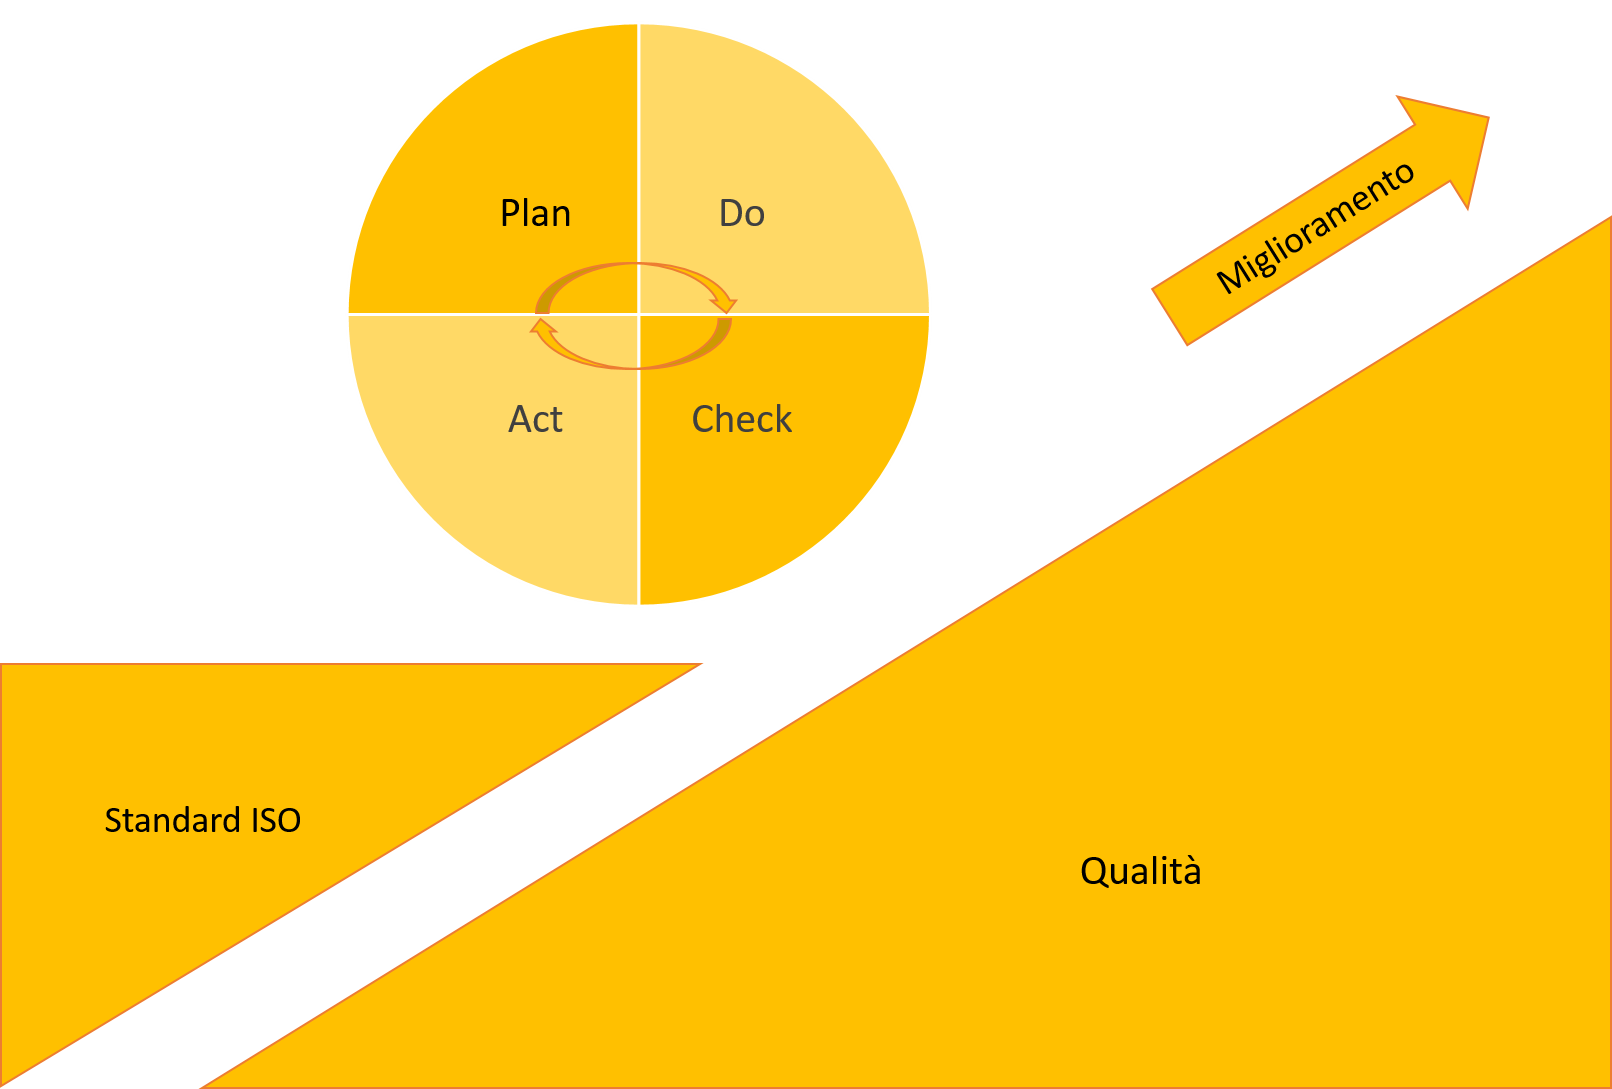
\includegraphics[width= 11.5cm]{immagini/pdca.png}
	\caption{Ciclo di Deming}
\end{figure}

Il ciclo PDCA\G\ è suddiviso in 4 fasi:

\begin{itemize}
	\item \textbf{Plan:} fase di pianificazione che definisce:
\begin{itemize}
	\item[-] Gli obiettivi da raggiungere;
	\item[-] Come svolgere le attività per conseguirli, tenendo in considerazione le risorse disponibili e le scadenze;
	\item[-] Le responsabilità di chi va ad eseguire le attività;
	\item[-] Le metriche per valutare i processi.
\end{itemize}
	
	\item \textbf{Do:} fase di implementazione ed esecuzione delle strategie progettate nella fase precedente;
	
	\item \textbf{Check:} fase di verifica nella quale vengono controllati i risultati della fase precedente (secondo le metriche fissate nella fase \textit{Plan}) e in cui si confrontano i prodotti effettivi con quelli attesi;
	
	\item \textbf{Act:} fase che prevede il miglioramento dei processi: utilizzando i risultati della verifica, si progettano modifiche ai processi per migliorarli. Nello svolgimento di questa attività viene tenuto conto delle \textit{best practice\G}. Tutte le decisioni prese in questa fase vengono implementate a partire dalla successiva fase di \textit{planning}.
\end{itemize}
Lo scopo di questo ciclo è il continuo incremento qualitativo del processo di sviluppo e, conseguentemente, del prodotto. L'appoggio agli \textit{standard} e alle \textit{best practice} permette di consolidare il livello raggiunto e di non retrocedere. Il miglioramento può progredire infinitamente nel tempo, data l'assenza di limiti fissati.

\subsection{Standard ISO/IEC 9126}

Lo standard ISO\G/IEC\G\ 9126 è stato creato con lo scopo di descrivere gli 
obiettivi qualitativi del prodotto e definire le metriche che possono misurare 
il raggiungimento di tali obiettivi. Vi sono infatti dei criteri suddivisi in tre 
aree:

\begin{itemize}
	\item \textbf{Qualità in uso:} è la qualità del prodotto \textit{software} 
	visto dall'utilizzatore, che ne fa uso in uno specifico contesto;
	\item \textbf{Qualità esterna:} è la qualità del prodotto 
	\textit{software} visto dall'esterno, quando viene eseguito e testato in un 
	ambiente di prova;
	\item \textbf{Qualità interna:} è la qualità del prodotto 
	\textit{software} visto dall'interno, facendo riferimento a 
	caratteristiche implementative, come l'architettura o il codice che ne 
	deriva.
\end{itemize}
Essendo inizialmente impossibile testare la qualità in uso, si è deciso di 
focalizzarsi sulla qualità interna ed esterna. Nello standard sono previste sei 
caratteristiche qualitative principali, suddivise a loro volta in 
sottocategorie che possono essere misurate quantitativamente:

\begin{itemize}
	\item \textbf{Funzionalità:} capacità del prodotto di fornire le funzioni richieste
	\begin{itemize}
		\item \textbf{Idoneità:} capacità del prodotto di fornire un insieme di funzioni appropriate per un'attività;
		\item \textbf{Accuratezza:} capacità del prodotto di fornire risultati 
		coerenti e corretti a seconda del grado di precisione richiesto;
		\item \textbf{Interoperabilità:} capacità interattiva del prodotto 
		\textit{software} con uno o più sistemi;
		\item \textbf{Sicurezza:} capacità del prodotto \textit{software} di 
		proteggere i dati e le informazioni, e a consentire solo a sistemi 
		autorizzati di fare modifiche;
		\item \textbf{Conformità funzionale:} capacità del prodotto 
		\textit{software} di essere aderente allo standard in materia di 
		funzionalità.
	\end{itemize} 
	
	\item \textbf{Affidabilità:} capacità del prodotto di garantire un livello di prestazioni adeguato
	\begin{itemize}
		\item \textbf{Maturità:} capacità del \textit{software} di evitare 
		fallimenti causati da errori;
		\item \textbf{Tolleranza agli errori:} capacità del \textit{software} 
		di mantenere un adeguato livello di prestazioni nonostante errori o 
		violazioni dell'interfaccia;
		\item \textbf{Capacità di recupero:} capacità del \textit{software} di 
		ristabilire un livello di \textit{performance} adeguato e di recuperare 
		dati in caso di errori;
		\item \textbf{Conformità di affidabilità:} capacità del prodotto 
		\textit{software} di essere aderente allo standard in materia di 
		affidabilità.
	\end{itemize}
	
	\item \textbf{Usabilità:} capacità del prodotto di essere facilmente comprensibile ed usabile, e di risultare interessante per l'utente
	
	\begin{itemize}
		\item \textbf{Intelligibilità:} capacità del \textit{software} di 
		permettere all'utente di capire se il prodotto è adeguato e se possa 
		essere utilizzato per dei compiti particolari;
		\item \textbf{Apprendibilità:} capacità del \textit{software} di 
		consentire all'utente di imparare ad utilizzare le sue funzionalità;
		\item \textbf{Operabilità:} capacità del \textit{software} di 
		consentire ai suoi utenti di essere usato;
		\item \textbf{Attrattività:} capacità del \textit{software} di creare 
		interesse negli utenti;
		\item \textbf{Conformità di usabilità:} capacità del 
		\textit{software} di essere aderente allo standard in materia di 
		usabilità.
	\end{itemize}
	
	\item \textbf{Efficienza:} capacità del prodotto di fornire prestazioni adeguate a seconda delle risorse utilizzate
	\begin{itemize}
		\item \textbf{Comportamento temporale:} capacità del \textit{software} 
		di dare una risposta in tempi di elaborazione adeguati, quando svolge 
		le sue funzionalità;
		\item \textbf{Utilizzo di risorse:} capacità del \textit{software} di 
		utilizzare le risorse adeguate per la sua esecuzione;
		\item \textbf{Conformità di efficienza:} capacità del 
		\textit{software} di essere aderente allo standard in materia di 
		efficienza.
	\end{itemize}
	
	\item \textbf{Manutenibilità:} capacità del prodotto di essere modificato e 
	aggiornato. Tali modifiche o aggiornamenti possono rispecchiare correzioni, 
	miglioramenti o adattamenti del \textit{software} nei confronti di cambiamenti ambientali, 
	di specifiche o delle funzionalità
	\begin{itemize}
		\item \textbf{Analizzabilità:} capacità del \textit{software} di poter 
		essere studiato per cercare difetti;
		\item \textbf{Modificabilità:} capacità del \textit{software} di 
		consentire l'implementazione di una qualche modifica;
		\item \textbf{Stabilità:} capacità del \textit{software} di evitare 
		errori o fallimenti causati da una o più modifiche;
		\item \textbf{Testabilità:} capacità del \textit{software} di 
		permettere la validazione di una versione modificata del 
		\textit{software};
		\item \textbf{Conformità di manutenibilità:} capacità del prodotto 
		\textit{software} di essere aderente allo standard in materia di 
		manutenibilità.
	\end{itemize}
	
	\item \textbf{Portabilità:} capacità del \textit{software} di poter essere 
	spostato in vari ambienti di lavoro
	\begin{itemize}
		\item \textbf{Adattabilità:} capacità del \textit{software} di essere 
		adattato a diversi ambienti senza necessitare di modifiche;
		\item \textbf{Installabilità:} capacità del \textit{software} di poter 
		essere installato in ambienti differenti;
		\item \textbf{Coesistenza:} capacità del \textit{software} di 
		coesistere con altri \textit{software} indipendenti condividendo delle 
		risorse;
		\item \textbf{Sostituibilità:} capacità del \textit{software} di poter 
		sostituire un \textit{software} simile che abbia le stesse funzionalità 
		e che sia nello stesso ambiente;
		\item \textbf{Conformità di portabilità:} capacità del prodotto 
		\textit{software} di essere aderente allo standard in materia di 
		portabilità.
	\end{itemize}
	
\end{itemize}
\newpage
\section{Resoconto delle attività di verifica}
\label{cap:Sezione 5 Resoconto delle attività di verifica}

\subsection{Riassunto delle attività di verifica}

\subsubsection{Revisione dei Requisiti}

Nel periodo antecedente alla consegna della documentazione sono state eseguite le attività di verifica dei processi e dei documenti redatti. Ogni documento è stato controllato tramite la tecnica del \textit{walkthrough} descritta nella sezione \hyperref[cap:sezione 2.8.2 Walkthrough]{2.8.2 Walkthrough}. Si sono riscontrati diversi errori che sono stati segnalati in modo informale ai redattori. Il gruppo è consapevole di non aver seguito la procedura descritta nella sezione \hyperref[cap: sezione 3.1 Comunicazione e risoluzione di anomalie]{3.1 Comunicazione e risoluzione di anomalie}. Pertanto si impegna a seguirla dalla prossima fase: Analisi di Dettaglio. Si precisa inoltre che nel corso di questa attività il gruppo non si è occupato di stilare la lista di controllo necessaria per la tecnica dell'\textit{inspection}. Infine, dopo la correzione dei documenti, si è provveduto a calcolare le metriche descritte nella sezione \hyperref[cap:sezione 2.9 Misure e metriche]{2.9 Misure e metriche}. \\
Il tracciamento dei requisiti è avvenuto grazie all'utilizzo di un \textit{software} realizzato appositamente dagli \textit{Amministratori} del gruppo. \\
I processi sono stati verificati utilizzando le metriche di processo descritte nella sezione \hyperref[cap: sezione 2.8.1 Metriche per i processi]{2.8.1 Metriche per i processi}. Sono quindi stati riportati i valori di BV e SV relativi a tutti i processi di ciascuna fase.

\subsection{Dettaglio delle verifiche tramite analisi}

\subsubsection{Documenti}
Riportiamo in questa sezione i valori degli indici Gulpease calcolati per ogni documento. Un documento è valido se e solo se rispetta le metriche descritte nella sezione \hyperref[cap:sezione 2.9.2 Metriche per i documenti]{2.9.2 Metriche per i documenti}.

\begin{table}[ht]
\centering
\begin{tabular}{|c|c|c|}
	\hline
	\textbf{Documento} & \textbf{Valore} & \textbf{Indice} \\ \hline
	\textit{Piano di Qualifica v1.0.0} & 54 & Superato \\ \hline
	\textit{Piano di Progetto v1.0.0} & 58 & Superato \\ \hline
	\textit{Norme di Progetto v1.0.0} & 56 & Superato \\ \hline
	\textit{Analisi dei Requisiti v1.0.0} & 60 & Superato \\ \hline
	\textit{Studio di Fattibilità v1.0.0} & 54 & Superato \\ \hline
	\textit{Glossario v1.0.0} & 50 & Superato \\ \hline
\end{tabular}
\caption{Indici Gulpease dei documenti}
\end{table}
La tabella mostra come i documenti rientrino tutti nel \textit{range} ottimale precedentemente definito. Rispettano pertanto il livello di leggibilità minimo desiderato.
\newpage

\subsubsection{Processi}

Qui vengono riportati i valori di SV e BV descritti nella sezione \hyperref[cap: 
sezione 2.8.1 Metriche per i processi]{2.8.1 Metriche per i processi}, 
per le attività nella fase di \textbf{Analisi dei Requisiti} che hanno portato alla stesura dei documenti.

\begin{table}[ht]
	\centering
	\begin{tabular}{|c|c|c|}
		\hline
		\textbf{Attività} & \textbf{SV} & \textbf{BV} \\ \hline
		
		\textit{Piano di Qualifica v1.0.0} & -30 € & -30 € \\ \hline
		\textit{Piano di Progetto v1.0.0} & 0 € & -30 € \\ \hline
		\textit{Norme di Progetto v1.0.0} & 0 € & -30 € \\ \hline
		\textit{Analisi dei Requisiti v1.0.0} & +50 € & +25 € \\ \hline
		\textit{Studio di Fattibilità v1.0.0} & +30 € & 0 € \\ \hline
		\textit{Glossario v1.0.0} & 0 € & 0 € \\ \hline
	\end{tabular}
	\caption{Metriche dei processi}
\end{table}

Complessivamente la fase di \textbf{Analisi} ha:

\begin{itemize}
	\item SV : +50€;
	\item BV : -65€.
\end{itemize}

Da questi indici si può notare che:

\begin{itemize}
	\item Grazie a una pianificazione accurata delle scadenze, le attività 
	sono state svolte nei tempi pianificati, alcune volte terminando in 
	anticipo rispetto alle date di fine prefissate;
	\item Il costo complessivo si è di poco discostato da quanto pianificato nel 
	\textit{Piano di Progetto v1.0.0}. La causa di questa variazione dei costi è imputabile alla poco esperienza del gruppo nel redigere tale tipologia di documenti.
\end{itemize}

\subsubsection{Esito delle revisioni}

Durante lo sviluppo del progetto vi saranno quattro revisioni da parte del Committente. Il Committente segnalerà problematiche che verranno riscontrate valutando globalmente l'andamento del progetto e di ogni singolo documento. Grazie a queste informazioni sarà possibile correggere gli errori commessi, al fine di procedere lungo delle attività lavorative che risultino corrette e verificate.

%\input {sections/nomesezione}
%\newpage

% ...

%\printglossaries

\end{document}
